\question{}
%\partQuestion{}

\listbeginx	% start 1st level question
	\item Bioelectric potentials are produced as a result of electrochemical activity of an excitable cell. In resting state where there is no stimulus, the cell is polarized.
	
	\translation{Daya bioelektrik dihasilkan dari kesan aktiviti elektrokimia sesuatu sel peka rangsang. Dalam keadaan rehat di mana tiada rangsangan, sel adalah terkutub.}
	
	\listbegin
		\item What is the typical value of cell membrane potential in resting state, and how it is measured?
		
		\translation{Apakah nilai daya membran sel dalam keadaan rehat, dan bagaimana ianya diukur?}
		
		\qmarks{2}
		
		\item Elaborate how the cell membrane potential maintained polarized in resting state.
		
		\translation{Huraikan bagaimana daya membran sel kekal terkutub sewaktu keadaan rehat.}
		
		\qmarks{8}
		
		\item Differentiate between absolute refractory period and relative refractory period, and why the value differs in ventricular cell?
		
		\translation{Bezakan di antara tempoh refraktori mutlak dan tempoh refraktori relatif, dan kenapa nilai ini berbeza untuk sel ventrikular?}
		
		\qmarks{5}
	\listclose 
	
%	\nextpage 
%	\clearpage 
	
	\item The simplest configuration of instrumentation amplifier (INA) is shown in \cref{fig:diffamp2}. 
	
	\translation{Tatarajah paling mudah bagi penguat instrumentasi (INA) ditunjukkan dalam \Cref{fig:diffamp2}.}
	
	\begin{figure}[H] % H means, to put figure here after the code		
		\centering
		%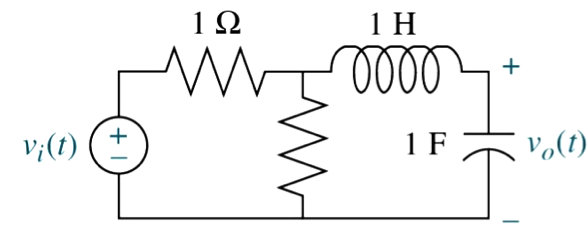
\includegraphics[width=0.5\textwidth]{testfig}
		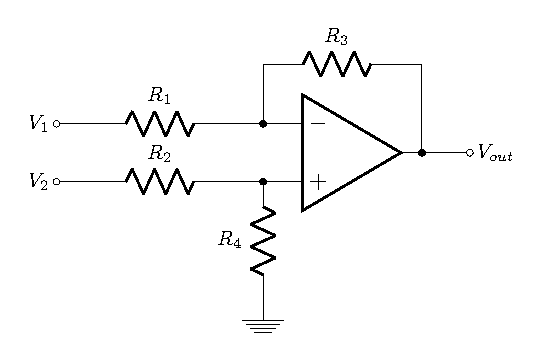
\includegraphics{diffamp}
		\caption{\rajah}
		\label{fig:diffamp2}
	\end{figure}

	% Table generated by Excel2LaTeX from sheet 'Sheet1'
	\begin{table}[H]
		\centering
		\caption{\jadual}	% no caption
		%\begin{tabularx}{220pt}{c c}
		\begin{tabular}{cc}
			\toprule
			% \toprule[1.5pt]
			\multicolumn{1}{l}{\textbf{Frequency}} & \multicolumn{1}{l}{\textbf{Impedance (Magnitude) ($\Omega$)}} \\
			\midrule
			5 Hz  & 20,000 \\
			10 Hz & 19,998 \\
			\vdots     & \vdots \\
			40 kHz & 602 \\
			50 kHz & 600 \\
			100 kHz & 600 \\
			\bottomrule
			%			\bottomrule[1.5pt]
		\end{tabular}
		%		\end{tabularx}%
		\label{table:freqmag}%
	\end{table}%	
	
	\listbeginx
	\item Prove that the differential gain, $A_d$ and common-mode gain, $A_{cm}$ of the INA are, 
	
	\translation{Buktikan bahawa gandaan kebezaan, $A_d$ dan gandaan ragam sepunya, $A_{cm}$ bagi INA adalah,}
	
	\begin{align*} 
		A_d &= \frac{1}{2}
		\left[
			\frac{R_4}{R_2}
				\left(\frac
					{1+\dfrac{R_3}{R_1}}
					{1+\dfrac{R_4}{R_2}}
				\right)
			+\frac{R_3}{R_1}
		\right] \\
		A_{cm} &= 
		\left[
			\frac{R_4}{R_2}
				\left(\frac
					{1+\dfrac{R_3}{R_1}}
					{1+\dfrac{R_4}{R_2}}
				\right)
			-\frac{R_3}{R_1}
		\right] 
	\end{align*}

	\qmarks{8}
	
	\answer{
		\begin{align*}
			 V_o &= A_dV_d + A_{cm}V_{cm} \\
			V_{cm} &= \frac{V_1+V_2}{2} & V_d &= V_2 - V_1 \\
			V_1 &= V_{cm}-\frac{V_d}{2} & V_2 &= V_{cm}+\frac{V_d}{2} 
		\end{align*}
		
		\begin{align*}
			V_2' &= \frac{R_4}{R_2+R_4}V_2 \\
			\frac{V_1-V_2'}{R_1} &= \frac{V_2' - V_o}{R_3} \\
			\frac{R_3}{R_1}\left(V_1 - V_2'\right) &= V_2' - V_o \\
			\frac{R_3}{R_1}V_1 + V_o &= \frac{R_3}{R_1}V_2' + V_2' \\
			V_o &= V_2'\left(\frac{R_3}{R_1} + 1\right) - \frac{R_3}{R_1}V_1\\
			&= \left[\frac{R_4}{R_2+R_4}\right]
				\left(\frac{R_3}{R_1}+1\right)V_2 - \frac{R_3}{R_1}V_1\\
			&= \left(\frac{R_4}{R_2+R_4}\right)
				\left(\frac{R_3}{R_1}+1\right)
				\left[V_{cm}+\frac{V_d}{2}\right] - \frac{R_3}{R_1}
				\left[V_{cm}-\frac{V_d}{2}\right]\\	
			&= \frac{V_d}{2}
				\left[
					\left(\frac{R_4}{R_2+R_4}\right)
					\left(\frac{R_3}{R_1}+1\right) + \frac{R_3}{R_1}
				\right] + 
				V_{cm}
				\left[
					\left(\frac{R_4}{R_2+R_4}\right)
					\left(\frac{R_3}{R_1}+1\right) - \frac{R_3}{R_1}
				\right]		
		\end{align*}

	Thus, differential gain, $A_d$ and common-mode gain, $A_{cm}$ is given by;
	
	\begin{align*} 
		A_d &= \frac{1}{2}
		\left[
			\frac{R_4}{R_2}
		\left(\frac
			{1+\dfrac{R_3}{R_1}}
			{1+\dfrac{R_4}{R_2}}
		\right)
			+\frac{R_3}{R_1}
		\right] \\
		A_{cm} &= 
		\left[
			\frac{R_4}{R_2}
		\left(\frac
			{1+\dfrac{R_3}{R_1}}
			{1+\dfrac{R_4}{R_2}}
		\right)
			-\frac{R_3}{R_1}
		\right] 
	\end{align*}
	\hfill Proven!
	\clearpage
	}

	\item  What is the expected output voltage if $R_4=R_3$ and $R_2=R_1$ where $R_2$ has 1\% tolerance. Justify your answer.
	
	\translation{Apakah voltan keluaran yang dijangka jika $R_4=R_3$ dan $R_2=R_1$ dimana $R_2$ mempunyai 1\% had terima. Wajarkan jawapan anda.}\\
	
	\answer{The output voltage will be summation of the differential voltage and common-mode voltage\\ \mbox{$V_o= A_dV_d + A_{cm}V_{cm}$} due to the mismatch of the $R_2$ resistor. 
	}
	
	\qmarks{2}
	
	\listclose	% close 2nd level question
\listclose	% close 1st level question